\documentclass[output=paper]{langsci/langscibook} 

\author{Karan Grewal\affiliation{University of Toronto} and Yang Xu\affiliation{University of Toronto}}

\title{Chaining algorithms and historical adjective extension}

\abstract{Natural language relies on a finite lexicon to express a potentially infinite set of ideas. This tension often results in the innovative reuse of existing words to describe emerging ideas. In this chapter, we take a computational perspective to examine how English adjectives extend their range over time to modify nouns and form previously unattested adjective-noun pairs. We hypothesize that how novel adjective-noun pairings emerge is non-arbitrary and follows a process of chaining, whereby novel noun referents for an adjective link to existing nouns modified by the same adjective that are close in semantic space. We test this proposal by exploring a set of probabilistic models that predict adjective-noun pairs from a historical text corpus (Google Books) that spans the past 150 years. Our findings across three diverse sets of adjectives support a chaining mechanism sensitive to local semantic neighbourhood -- formulated as an exemplar model of categorization similar to the Generalized Context Model. These findings mirror existing work on chaining in the historical growth of grammatical categories. We discuss the limitations and implications of our approach toward a general theory of word meaning extension in natural language.}

\begin{document}
\SetupAffiliations{mark style=none}
\maketitle


\section{Introduction}

Natural language relies on a finite lexicon to express a potentially infinite set of ideas. One result of this tension is the innovative reuse of existing words~\citep{ramiro2018}. Here we explore how English adjectives extend their range over time to modify novel nouns and ask whether there are principled mechanisms in the historical process of adjective extension.\footnote{See \citet{grewal2020chaining} for a shorter conference version of this work.}

The topic of adjective-noun composition has been discussed in the computational literature. Existing studies have explored which adjective-noun pairings are considered plausible~\citep{lapata1999}, and how adjectives can be combined with nouns sensibly either via probabilistic models~\citep{lapata2001} or through ontological constraints~\citep{schmidt2006}. Recent work has also suggested that adjective-noun composition can be modelled using vector-space models such as Word2Vec~\citep{mikolov2013-distributed}. In these studies, adjectives are considered to be linear operators that act on nouns in a vector space that impose linear transformations~\citep{baroni2010, boleda2013, vecchi2013, vecchi2017} or conform to additive compositional models~\citep{zanzotto2010}. Despite this extensive line of work, sparse computational research has considered the dimension of time in the investigation of adjective-noun composition.

Independent research in historical linguistics has explored adjective extension from the perspective of semantic change. In particular, \citet{williams1976} studied meaning change in synaesthetic adjectives and found that sensory terms such as those pertaining to sound, touch, and smell exhibit regular semantic shift such that words from the same sensory domain tend to undergo parallel change in meaning. For instance, \citet{williams1976} showed how adjectives that originally described the sense of touch have since extended to describe color (e.g., {\it warm cup} $\rightarrow$ {\it warm color}), and adjectives that originally described color have later extended to describe ideas associated with sound (e.g., {\it clear blue} $\rightarrow$ {\it clear voice}). This line of inquiry takes an empirical approach to characterize meaning change in adjectives from a focused semantic domain, but to our knowledge the more general problem of how adjectives extend their range to describe novel noun referents has not been treated formally or explored at scale.

We investigate whether adjective extension might follow non-random processes that make novel adjective-noun pairings yet to emerge in a linguistic community predictable. Our view is that novel adjective-noun pairings provide an incremental way of extending the referential range of adjectives, and word meaning extension or  semantic change might result from this process (e.g., consider meaning extension in the adjective \textit{cold} reflected in a chain of different noun context: \textit{cold food} $\rightarrow$ \textit{cold person} $\rightarrow$ \textit{cold war}). It is conceivable that pairing with novel nouns does not necessarily entail semantic change in an adjective (e.g., \textit{cold Gatorade} does not entail semantic change in \textit{cold} which had the meaning `low-temperature', even though \textit{Gatorade} might appear as a novel item to pair with \textit{cold} at some point in history), and our main focus here is to characterize the general mechanisms of an adjective's extension over time -- with or without  semantic change. 

Figure~\ref{fig:intro} illustrates that historical adjective-noun pairings can often be subject to non-linguistic or external influences which make them non-trivial to predict. For instance, the emergence of {\it vegan} is largely a cultural product, and different adjectives have been extended to modify this noun over time presumably as a result of cultural development. Our premise is that despite the historical  adjective-noun pairings may be subject to socio-cultural influences, language users must somehow choose adjectives  sensibly to describe nouns so that the novel pairings can be related to the original meaning of the adjectives. For this reason, we expect the historical processes of adjective extension to follow non-arbitrary paths.  


\begin{figure}[t!]
\begin{center} 
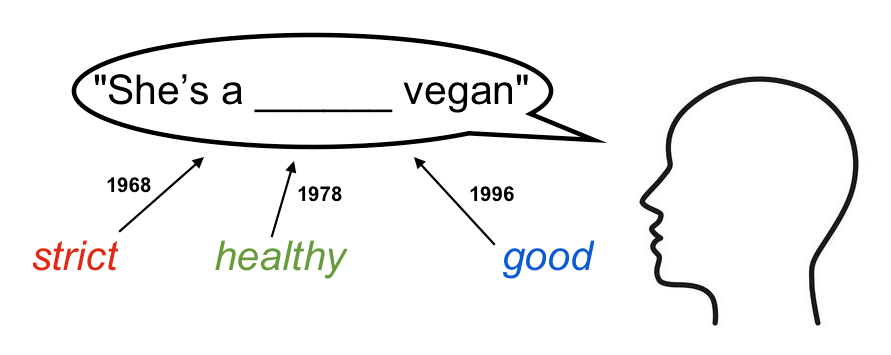
\includegraphics[width=4.5in]{figures/GREWAL_intro.png}
\end{center}
\caption{Example adjectives that emerged to describe {\it vegan} over the past half century.} 
\label{fig:intro}
\end{figure}


We formulate adjective extension as a temporal prediction problem: Given adjective-noun pairings at historical time $t$, can we predict novel adjective-noun pairings into the future at $t + \Delta$? We ground our  work in cognitive linguistic theories of chaining, which have been proposed and recently demonstrated as important cognitive mechanisms for historical word meaning extension~\citep{lakoff1987,malt1999,bybee1994evolution,sloman,xu2016,ramiro2018,habibi}. A consistent finding from these studies is that chaining as an extensional mechanism depends on semantic neighbourhood density, highlighting the fact that historical word meaning extension tends to follow incremental as opposed to abrupt processes. In our study, we consider each adjective as a linguistic category and explore different mechanisms of chaining to predict how adjective categories grow to modify nouns that they have not previously been paired with. We next describe the theory of chaining and related  work on word meaning extension.


\section{Theory of chaining and word meaning extension}

The proposal of semantic chaining is rooted in cognitive linguistic work on categories, or more specifically, radial categories~\citep{lakoff1987}. By this view, chaining is a process of meaning extension whereby novel items link to existing items of a linguistic category due to proximity in semantic space. This process leads to chain-like semantic structures, and \citet{lakoff1987} has considered it a key mechanism for growing radial categories or semantic networks, i.e., how categories grow ``spokes'' of meaning from a central core meaning. \citegen{lakoff1987} original work discusses chaining in a number of exemplary domains such as the grammatical categories of classifiers in Japanese and Dyirbal (an Australian aboriginal language), and  prepositions such as how the English spatial term \textit{over} extends over a wide variety of spatial (e.g., \textit{over the hill}) and metaphorical context (e.g., \textit{over the moon}). Later work also discusses chaining in the grammar evolution of tense, modality, and aspect systems~\citep{bybee1994evolution}, container naming~\citep{malt1999}, and metonymical semantic shift~\citep{hilpert2007chained}. These studies have broadened the view of chaining toward a generic mechanism for grammatical and semantic changes in language, although they do not provide a formal account for the processes of chaining or test this idea comprehensively against historical corpus data.


Extending the cognitive linguistic accounts of chaining, recent work has explored formal approaches to chaining in several aspects. \citet{sloman} and \citet{xu2016} have developed computational models of chaining and tested the extent to which these models account for the extension of container names such as \textit{bottle} and \textit{jar}. Their findings suggest that chaining depends on semantic neighbourhood density, and more specifically nearest-neighbour models of chaining tend to best account for the empirical data. \citet{ramiro2018} extend this work to examine whether similar models of chaining might explain the historical emergence of senses (or word sense extension) in English words over the past millennium, e.g., how \textit{face} might extend from `body part' to senses including `front surface (of an object)', `facial expression', and `defy danger'. Their work confirms the earlier finding that chaining relies on semantic neighbourhood density, and senses tend to emerge by linking those that are close in semantic space. 


More recent work has built on these computational studies to investigate the historical growth of grammatical categories, and particularly numeral classifiers commonly used in East Asian languages~\citep{habibi}. This work has examined a suite of probabilistic models of chaining and found chaining to be best captured by an exemplar model, also known as the Generalized Context Model in the psychological literature of categorization~\citep{nosofsky1986}. By this view, chaining in linguistic categories reflects an exemplar-based process of extension that mirrors those found in other aspects of language change including phonetics, morphology, word senses, and constructions~\citep{skousen89,pierrehumbert2001exemplar,keuleers08,bybee2013usage,ramsey17}.




Here we examine chaining through the lens of the exemplar theory but in a new domain: the case of historical adjective extension in English. Analogous to how numeral classifiers (e.g., in Mandarin Chinese) extend toward novel nouns, English adjectives also extend to modify novel noun referents. If the exemplar view represents a general mechanistic account for the growth of linguistic categories, it should explain the historical extension of adjective categories.

Figure~\ref{fig:chainexample} illustrates the exemplar theory of chaining with two example adjectives and a dimension-reduced semantic space of their noun referents, data for which were taken from the Google Books corpus~\citep{michel2011quantitative} during the 1880s. The two adjectives \textit{wrong} and \textit{troubled} are closely related in semantic space in the 1880s and share noun referents (labelled in purple) such as \textit{war} and \textit{humanity}. The emergent or query noun \textit{slavery} has not appeared in close context with either adjective prior to the 1880s but is in semantic proximity of their noun referents. The exemplar view of chaining postulates that the linguistic category having a higher local semantic similarity (or neighbourhood density) to a novel referent is more likely to attract that item, and when this process repeats over time chain-like category structures may result in semantic space. Here, \textit{wrong} has a higher neighbourhood density (with its noun referents labelled in red) to \textit{slavery} in comparison to \textit{troubled} (with its noun referents labelled in blue), namely that the existing noun referents of \textit{wrong} are closer in semantic space to the query noun than those of \textit{troubled}. The exemplar view of chaining thus predicts that \textit{wrong} is a more likely adjective candidate to be paired with \textit{slavery}, which aligns with the empirical data. We seek to evaluate the extent to which the exemplar model of chaining accounts for historical adjective extension, and if it is better or worse than alternative accounts for the chaining process.


\begin{figure}
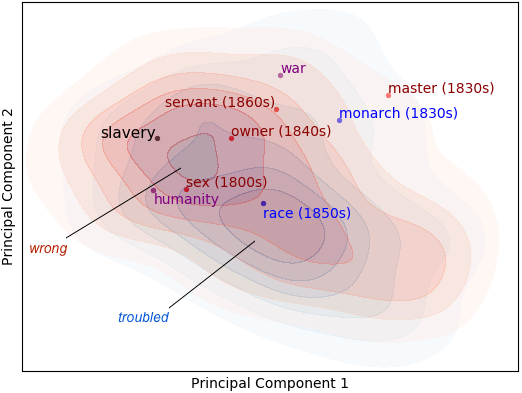
\includegraphics[width=4in]{figures/GREWAL_example.png} 
\caption{An illustration for the exemplar view of semantic chaining~\citep{habibi} using two example adjectives \textit{wrong} and \textit{troubled}. The semantic space is constructed from the first 2 principal components in the Principal Components Analysis on the diachronic Word2Vec embeddings from the 1870s~\citep{hamilton-etal-2016-diachronic}. Nouns labelled in purple (e.g., {\it humanity}, {\it war}) are shared context of the two adjectives. Nouns labelled in red (e.g., {\it master}, {\it servant}, {\it owner}, {\it sex}) and blue (e.g., {\it monarch}, {\it race}) are contexts that co-occurred more often with \textit{wrong} and \textit{troubled} respectively up to the 1880s. The contours represent probability distributions of nouns co-occurring with each of the two adjectives, constructed by kernel density estimation.}\label{fig:chainexample}
\end{figure}

\section{Computational formulation of theory}


We formulate adjective extension as a temporal categorization problem and explore the process of chaining via a suite of models that predict adjective-noun pairings over time. The probabilistic formulation we describe here follows existing work on chaining and the extension of numeral classifiers~\citep{habibi}.

\subsection{Probabilistic formulation}\largerpage[-1]


Given an emergent query noun $n^*$ at a future time $t + \Delta$ and a finite set of adjectives $\mathcal{A}$, we seek to predict which adjective(s) $a \in \mathcal{A}$ would be most appropriate for describing $n^*$ at time $t + \Delta$ based on the historically attested adjective-noun pairings at current time $t$.\footnote{In our formulation of the prediction problem, we consider an adjective-noun pair to be novel if (1) the noun itself is novel or (2) the pairing has not been attested in history.} We cast this problem as  probabilistic inference over the space of adjectives for a query noun $n^*$:
\begin{equation}
    p\left(a|n^*\right)^{(t + \Delta)} \propto p\left(n^*|a\right)^{(t)} p\left(a\right)^{(t)}. \label{framework}
\end{equation} 


The posterior term $\smash{p\left(a|n^*\right)^{(t + \Delta)}}$ relies on two sources of information to predict the choice of adjective(s) for $n^*$: (1) a likelihood function $\smash{p\left(n^*|a\right)^{(t)}}$ that specifies the semantic proximity of $n^*$ to an adjective $a$ given knowledge of its existing noun referents at time $t$, and (2) a prior distribution $\smash{p\left(a\right)^{(t)}}$ that captures the a priori belief or probability of choosing an adjective $a$ from the current lexicon without considering its semantic relation to $n^*$. In both our formulations of the likelihood and the prior, we focus on type-based representations of adjective-noun co-occurrence frequencies and adjective frequencies. Token-based representations have  been explored and shown to be inferior in accounting for the historical growth of classifier categories in related recent work~\citep{habibi}.



\subsection{Likelihood function}

We describe a suite of models to explore a space of possible candidates for the likelihood function. Each of these models postulates a different mechanism of chaining that links existing noun referents of an adjective to a novel noun that appears at a future time. We use $\smash{\{n\}_a^{(t)}}$ to denote the semantic embeddings for the set of nouns that co-occur with adjective $a$ at current time $t$, i.e., the semantic representation for the collective set of noun referents for adjective category $a$. Figure \ref{fig:models} provides an illustration for the representative chaining models that we describe in the following subsections. 



\begin{figure}
\begin{subfigure}[b]{.32\textwidth}
  \centering
  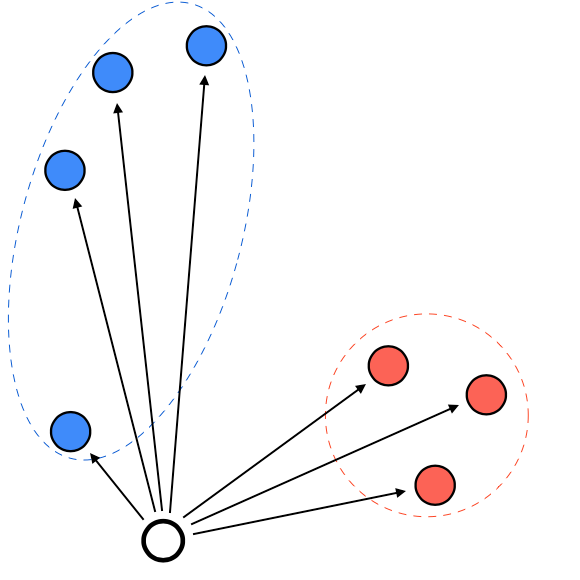
\includegraphics[width=.7\linewidth]{figures/GREWAL_exemplar.png}
  \caption{exemplar}
\end{subfigure}\begin{subfigure}[b]{.32\textwidth}
  \centering
  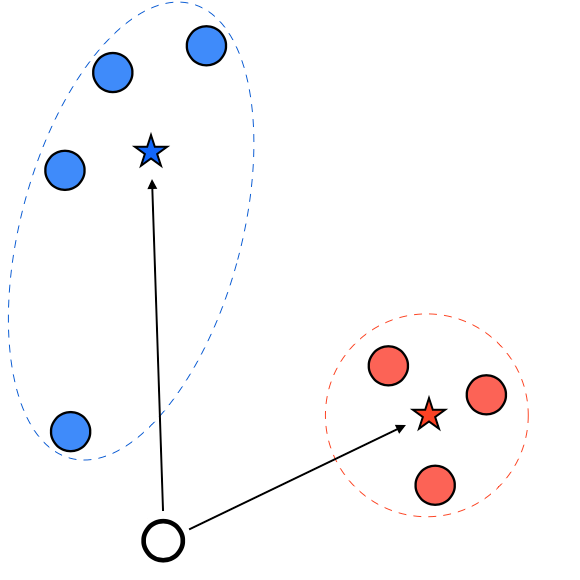
\includegraphics[width=.7\linewidth]{figures/GREWAL_prototype.png}
  \caption{prototype}
\end{subfigure}\begin{subfigure}[b]{.32\textwidth}
  \centering
  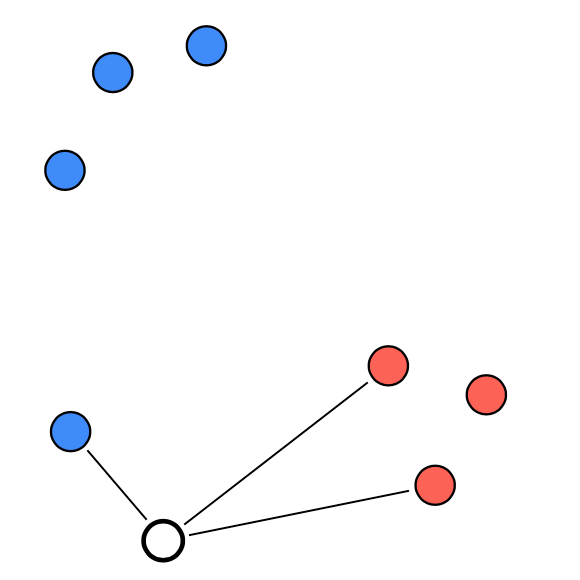
\includegraphics[width=.7\linewidth]{figures/GREWAL_nn.png}
  \caption{$k$-nearest neighbours, $k=3$}
\end{subfigure}
\caption{An illustration of representative chaining models for the likelihood function. The empty circle represents the stimulus or the query noun $n^*$. Red circles represent nouns that are attested to have paired with one particular adjective, and blue circles represent nouns that are attested to have paired with an alternative adjective (in reality, a noun can pair up with multiple adjectives). The dotted lines indicate the noun referent space for a given adjective. The stars represent the prototypes under the prototype model. The lines indicate the influence of existing (exemplar) nouns to the query noun as specified in each model of chaining.}
\label{fig:models}
\end{figure}

\subsubsection{Exemplar model}

The first likelihood function we consider is based on the exemplar theory which is  discussed in the psychological literature of categorization~\citep{nosofsky1986}. Here each noun $\smash{n \in \{n\}_a^{(t)}}$ is treated as an exemplar for an adjective $a$.

The exemplar view of chaining postulates that a query noun should be linked to an adjective category where the noun exemplars are most proximal in semantic space. As such, a novel noun is pulled or attracted to the adjective category that has the highest local semantic density around that noun. The likelihood term between $n^*$ and adjective $a$ is thus proportional to the weighted sum of similarities between $n^*$ and the noun exemplars of $a$:

\begin{equation}
    p(n^*|a)^{(t)} \propto \frac{1}{h\left| \{n\}_a^{(t)} \right|} \sum_{n \in \{n\}_a^{(t)}} \text{sim}(n^*, n) \label{exemplar}
\end{equation}

The similarity function $\text{sim}(\cdot, \cdot)$ measures how similar two nouns are and is defined as the exponentiated negative distance in semantic space which assigns differential weights to exemplars based on their relative distances to the query (higher similarities for more proximal exemplars):

\begin{equation}
    \text{sim}(n^*, n) = \text{exp}\left(-\frac{d(n^*, n)^2}{h}\right)
\end{equation}


$d\left(\cdot, \cdot\right)$ measures the Euclidean distance between nouns and $h$ is a kernel parameter that we learn from data. The choice of the exemplar model and the similarity formulation is grounded in work on Generalized Context Model~\citep{nosofsky1986}, which has recently been shown to predict the historical extension of Chinese numeral classifiers~\citep{habibi}. Here we examine whether the same exemplar-based processes of chaining might explain historical adjective extension. This model is also equivalent to performing kernel density estimation in semantic space defined by the likelihood function, and thus we use a kernel parameter $h$ in the similarity function and normalize the term by dividing the resulting sum by $h$. 




\subsubsection{Prototype model}\largerpage

Motivated by earlier psychological work on prototype theory~\citep{rosch1975} and related recent work on few-shot learning~\citep{snell2017}, we consider an alternative view of chaining based on category prototypes. Each adjective $a$ is represented by a prototype at time $t$ that captures the ``gist'' of noun referents for that category. We operationalize the prototype as the expectation of all exemplars within a category:

\begin{equation}
    \vec{\text{p}}_a = \mathbb{E}\left[n \in \{n\}_a^{(t)}\right] = \frac{1}{\left|\{n\}_a^{(t)}\right|} \sum_{n \in \{n\}_a^{(t)}} n \label{proto}
\end{equation}

The likelihood function postulates a chaining mechanism that links a query noun to the adjective that has the closest prototype in semantic space:

\begin{equation}
        p(n^*|a)^{(t)} \propto \text{sim}(n^*, \vec{\text{p}}_a) = \text{exp}\left(-\frac{d(n^*,\vec{\text{p}}_a)^2}{h'}\right) \label{prototype}
\end{equation}

Similar to the exemplar model, we use a kernel parameter $h'$ that controls how quickly similarity scales with respect to the semantic distance between the query noun and the prototype. This model can behave differently from the exemplar model of chaining: even if a query noun is closer to the prototype of one adjective over an alternative adjective, a small set of exemplars closest to that noun can pull the query item to the alternative category (see~\citealp{habibi} for a simulation that compares the properties of the exemplar and prototype models of chaining).   

We also consider a variant of the prototype model in which the prototype representation for each adjective category remains static over time. That is, \[\vec{\text{p}}_a = \vec{\text{p}}_a^{(t_0)}\] for all $t > t_0$ where $t_0$ is the initial time of investigation.
We refer to this variant as the progenitor model.


\subsubsection{$k$-nearest neighbours model}

In addition to the exemplar and prototype models, we consider a family of models based on $k$-nearest neighbours ($k$-NN). In a Bayesian framework, the  $k$-NN likelihood of $n^*$ pairing up with adjective $a$ is proportional to whether its $k$ closest neighbours $n_1, \ldots, n_k$ previously paired up with $a$, and inversely proportional to the size of category $a$:


\begin{equation}
    p(n^*|a)^{(t)} \propto \frac{1}{\left| \{n^*\}_a^{(t)} \right|} \sum_{j=1}^k I ( n_j \in \{n\}_a^{(t)} )
\end{equation}

Here the sum is over the $k$ nouns closest to $n^*$ in semantic space.
When this likelihood is combined with the prior, the $k$-NN posterior probability amounts to $n^*$'s $k$ closest neighbours voting for each of the adjectives that they previously paired up with.

This formulation of $k$-NN can be viewed as a ``hard version'' of the exemplar model where $k$ is a discrete analog of the kernel parameter $h$.
We report $k=1$ and $k=10$ in our experiments.


\subsection{Prior distribution}

We formulate a type-based prior $\smash{p\left(a\right)^{(t)}}$ which specifies how likely adjective $a$ is to be paired with any noun based on the set size of its noun referents at time $t$. This prior formulation predicts that $a$'s probability of appearing in a novel adjective-noun pairing is directly proportional to the number of unique nouns it has previously paired up with:

\begin{equation}
    p(a)^{(t)} = \frac{\left| \{n\}_a^{(t)} \right|}{\sum_{a' \in \mathcal{A}} \left| \{n\}_{a'}^{(t)} \right|}
\end{equation}


The rationale behind this choice of prior is as follows: if semantic chaining underlies the emergence of novel adjective-noun pairs, then adjectives that have paired with more nouns would have a higher a priori probability of attracting a query noun $n^*$ via linking it to semantically similar nouns which are more likely to have previously co-occurred with $a$ \citep{luo2018}.
This rich-get-richer process is also supported by work on how semantic networks grow through preferential attachment \citep{steyvers2005}.

This category-size-based prior serves as our baseline model when making adjective predictions for $n^*$ at time $t + \Delta$, where $\smash{p\left(a|n^*\right)^{(t + \Delta)} = p\left(a\right)^{(t)}}$. We focus on the type-based representation as opposed to token frequencies because work from \citet{habibi} has shown that a type-based prior worked better than a token-based prior in predicting the extension of grammatical categories.



\subsection{Semantic space}
\label{semanticspace}

To construct a semantic space for the nouns, we use word embeddings, particularly Word2Vec, commonly used for distributed semantic representation in natural language processing~\citep{mikolov2013-distributed}. We choose this construction of semantic space partly because it has been demonstrated to be effective in predicting grammatical category extension~\citep{habibi}. However, adjective usage is likely to entail a semantic representation richer than purely linguistic information, and future work should explore alternative methods for constructing semantic space such as those based on perceptual features and lexical taxonomic structures.

Since the word co-occurrence distributions are constantly changing over time, our semantic representations (of nouns) also need to be updated accordingly. For this reason, we use diachronic (or historical) Word2Vec embeddings~\citep{hamilton-etal-2016-diachronic} where at each time $t$, the embedding for a noun is based on its co-occurrence profiles at time $t$, relatively independent to future co-occurrences. In this respect, the predictions made by our models are in some sense ``zero-shot'', or deprived of semantic information into the future.


\section{Data}
\label{section:data}

\begin{sloppypar}
We extracted a large database of historical adjective-noun pairings over the past 150 years (1850--2000).
We collected these data from the Google Books corpus~\citep{michel2011quantitative} which contains sentence fragments from historical books over the past five centuries. Within Google Books, the English All ({\sc EngAll}) corpus accounts for $8.5 \times 10^{11}$ tokens and roughly 4\% of all books ever published. The diversity and size of the {\sc EngAll} corpus should reflect how the English language has been used over the past centuries, which makes our adjective-noun co-occurrence dataset suitable for evaluating hypotheses about chaining.
\end{sloppypar}

We collected adjective-noun co-occurrence counts from the {\sc EngAll} corpus. First, we extracted all bigrams from the {\sc EngAll} corpus in which the first token is an adjective and the second is a noun (by part-of-speech tags specified in the data) along with the corresponding timestamp. Since the corpus is likely to contain noise, we standardized the set of nouns and adjectives by only considering those present in WordNet~\citep{miller1995wordnet}, which yields approximately 67k nouns and 14k adjectives.

We collapsed raw co-occurrence counts into decadal bins by choosing $\Delta = 10 \text{ years}$.
This yielded our adjective-noun pairings dataset which consists of entries of the form ($a$, $n$, count, $t$).
In each decade $t$, we used a Word2Vec language model pre-trained on historical text (i.e., digitized books from Google Books) for the semantic representation. For our analyses, we worked with a subset of the collected data (discussed in the next section), due to both considerations of sampling diversity and computational feasibility. To construct semantic representations across decades, we used diachronic Word2Vec embeddings which were trained using the {\sc EngAll} corpus.
\citep{hamilton-etal-2016-diachronic} also chose to construct diachronic Word2Vec embeddings decade-by-decade for similar reasons.

We now describe three adjective sets $\mathcal{A}$.
The purpose of evaluating our models on three different adjective sets is to obtain representative samples of the adjectives, and to ensure our hypotheses are robust to the choice of adjectives.

\begin{description}
\item[{\normalfont(1)} Frequent adjectives.] We use multiple ways to construct $\mathcal{A}$ such that it covers a broad scope and show our results are reproducible and agnostic to choice of adjectives.
To construct a set of 200 adjectives that cover a broad range of descriptions, we first collected word vectors of all adjectives in the Google Books corpus using a pre-trained Word2Vec model.
Next, we clustered the adjectives into 20 clusters and picked 10 adjectives from each to construct our set $\mathcal{A}$ of 200 adjectives. We applied this clustering procedure to obtain a feasibly large yet diverse set of adjectives for the analyses, and we used the $k$-means algorithm for clustering. Adjectives were sampled from each cluster based on their usage frequencies, and only considered against other adjectives within the same cluster during sampling.
We refer to this set as {\sc Frq-200}, with examples shown in Table \ref{table:clusters}.


\item[{\normalfont(2)} Random adjectives.] To ensure that the sampling scheme for choosing $\mathcal{A}$ is not biased towards token frequencies, we also constructed another set of 200 adjectives by repeating the clustering step  described above, but we replaced frequency sampling with uniform sampling.
We refer to this dataset as {\sc Rand-200}.
As Table \ref{table:clusters} shows, adjectives drawn from the same cluster are semantically similar between {\sc Frq-200} and {\sc Rand-200}, but less common in the latter set.

\item[{\normalfont(3)} Synaesthetic adjectives.] We also consider the third set of {\it synaesthetic adjectives} ({\sc Syn-65})  defined by \citet{williams1976}, as a more focused domain that is known to undergo semantic change. This set includes 65 adjectives that exhibit regular semantic shift historically. We will refer to this set as {\sc Syn-65}.\footnote{There are in fact 64 unique adjectives in this set and WordNet captures 61 of these adjectives.
See \citet{williams1976} for a comprehensive list.}
\end{description}

Data and code from our analyses are available at \url{https://git.io/JqeyK}.%%\url{https://github.com/karangrewal/adjective-extension}.

\begin{table}
\caption{A comparison of some adjectives in {\sc Frq-200} and {\sc Rand-200} grouped according to the cluster they were drawn from.
Notice that the clusters (per column) align semantically, however the adjectives in {\sc Frq-200} are more frequently represented in the English lexicon than those in {\sc Rand-200}.}
\label{table:clusters} 
\begin{tabular}{llll}
\lsptoprule
{\sc Frq-200} & {\sc Rand-200} & {\sc Frq-200} & {\sc Rand-200} \\
\midrule
{\it Asian} & {\it Hungarian} & {\it polite} & {\it chatty} \\
{\it Christian} & {\it Thai} & {\it intelligent} & {\it unorthodox} \\
{\it American} & {\it Cornish} & {\it passionate} & {\it amiable} \\
{\it European} & {\it Catalan} & {\it energetic} & {\it communicative} \\
\lspbottomrule
\end{tabular}
\end{table}




\section{Results}

We present results in two steps. First, we examine the set of chaining algorithms described on novel adjective-noun pairings that appeared during 1850--2000, and we evaluate whether the exemplar model would better predict these data than the alternative models. Second, we perform a more focused analysis to examine whether the chaining algorithms predict extensional patterns in adjectives that show most and least semantic change over the past 150 years.

\subsection{Evaluation of chaining algorithms} \label{sec:modeval}

We evaluated the set of chaining algorithms on their ability to predict which adjectives $a \in \mathcal{A}$ would pair up with a given noun $n^*$ in decade $t + \Delta$ given  information about $n^*$ up to and including decade $t > t_0$, where $t_0$ is the base decade.
This information includes co-occurrences between all nouns $n$ and adjectives $a \in \mathcal{A}$ at or before decade $t$, as well as time-dependent word embeddings at each decade taken from \citet{hamilton-etal-2016-diachronic}.
We chose $t_0$ as the 1840s and built a base lexicon from adjective-noun co-occurrences between $t_0$ and the 2000s.
The 1860s was the first decade for which we report model prediction, and we used the 1850s as our ``training decade'' to estimate the kernel parameters for the exemplar and prototype models.

We define pairings ($a$, $n^*$) to be novel in decade $t + \Delta$ if and only if (i) $a$ co-occurred with $n^*$ in decade $t + \Delta$ beyond a certain threshold (which we set to~2), and (ii) $a$ never appeared with $n^*$ beyond that threshold in any decade $t' < t$.
Using these criteria allowed us to eliminate noise from co-occurrence statistics.
Given a noun $n^*$, each model's output was a categorical distribution $\smash{p\left(a|n^*\right)^{(t + \Delta)}}$ over all adjectives $a \in \mathcal{A}$.
The model was then scored on its precision accuracy on the set of adjectives that first co-occurred with $n^*$ in decade $t + \Delta$.
That is, if $n^*$ co-occurred with $m$ new adjectives in $\mathcal{A}$ in decade $t + \Delta$, we took the top $m$ adjectives with the highest posterior probabilities that had not previously co-occurred with $n^*$ as the set of retrieved positives. This evaluation metric calculates the percentage of correct predictions a model makes, and it is identical to the metric used in previous work for the prediction of historical extensions of classifier categories~\citep{habibi}. We report the total precision for all models and  use this metric as an objective function to learn the kernel parameters from the initial training decade. We consider two types of predictive tasks when making predictions for noun $n^*$ in decade $t$: taking as ground truth adjectives that co-occur with $n^*$ (1) specifically in the immediate future decade $t + \Delta$, and (2) all future decades $t' > t$ up to the terminal decade 1990s.

We summarize results from our experiments for the three differently sampled adjective sets $\mathcal{A}$.
As Figure \ref{fig:aggregate} shows, the exemplar model has the highest predictive performance, followed closely by the 10-NN and prototype models.
The exemplar, prototype, and 10-NN models perform substantially better than the baseline. These results provide evidence that chaining may rely on mechanisms sensitive to semantic neighbourhood density, best captured by the exemplar model. We also observed that the 10-NN model did not perform better than the exemplar model as the kernel parameter is a continuous analog of $k$ and is optimized for precision, but increasing $k$ in $k$-NN beyond 10 did help to improve model prediction suggesting that local neighbourhood density matters in predicting adjective extension.
The progenitor model, a variant of the prototype model with static prototypes determined in decade $t_0$, is considerably worse than the prototype model with a moving prototype.
This relationship between the prototype and progenitor models that we observe indicates that if the prototype model is the closest underpinning of adjective extension, then $\smash{\{n\}_a^{(t)}}$ largely influences which nouns adjective $a$ will extend to and that each adjective category ``center'' updates once novel adjective-noun pairings are formed. We also observed that the baseline or prior model performed worse than the exemplar and prototype models, suggesting that semantic relations matter in adjective-noun pairing, above and beyond the size-based adjective priors.\largerpage



\begin{figure}
\begin{subfigure}{.32\textwidth}
  \centering
  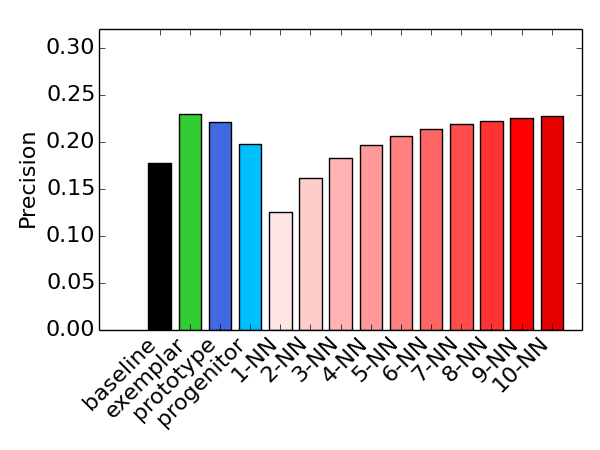
\includegraphics[width=.96\linewidth]{figures/GREWAL_aggregate_precision_frq200.png}
  \caption{\sc Frq-200}
\end{subfigure}\begin{subfigure}{.32\textwidth}
  \centering
  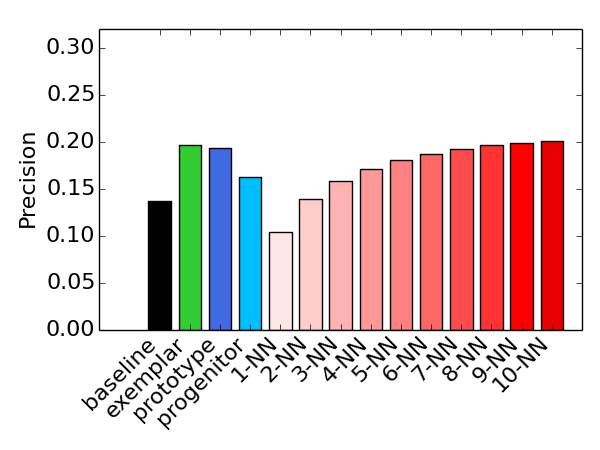
\includegraphics[width=.96\linewidth]{figures/GREWAL_aggregate_precision_rand200.png}
  \caption{\sc Rand-200}
\end{subfigure}\begin{subfigure}{.32\textwidth}
  \centering
  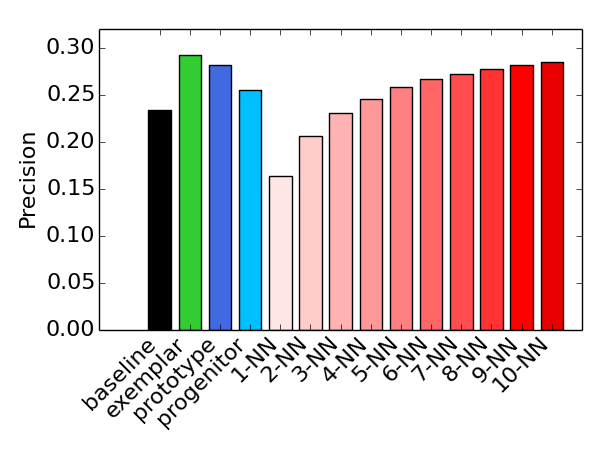
\includegraphics[width=.96\linewidth]{figures/GREWAL_aggregate_precision_syn65.png}
  \caption{\sc Syn-65}
\end{subfigure}
\caption{Aggregate precision accuracy for all models (including $k$-NN from $k = 1$ to $k = 10$) across all time periods on each of our three adjectives sets.}
\label{fig:aggregate}
\end{figure}



Further results with year-over-year accuracy breakdowns are shown in Figure \ref{fig:accuracy}.
The predictive accuracy falls in later decades since there are fewer novel adjective-noun pairings to predict. Our results hold generally across the three adjective sets, and they suggest that semantic neighbourhood density is an important factor contributing towards adjective extension as the exemplar and \mbox{10-NN} models achieve overall better predictive accuracy over the other alternative models. 




\begin{figure}[t]
\begin{subfigure}{\textwidth}
  \centering
  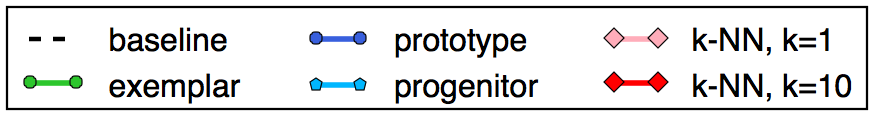
\includegraphics[width=.50\linewidth]{figures/GREWAL_legend.png}
\end{subfigure}
\begin{subfigure}{.32\textwidth}
  \centering
  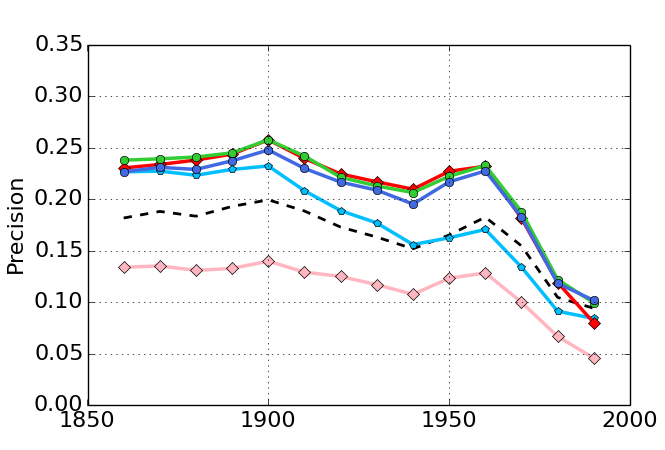
\includegraphics[width=.98\linewidth]{figures/GREWAL_precision_frq200.png}\\
  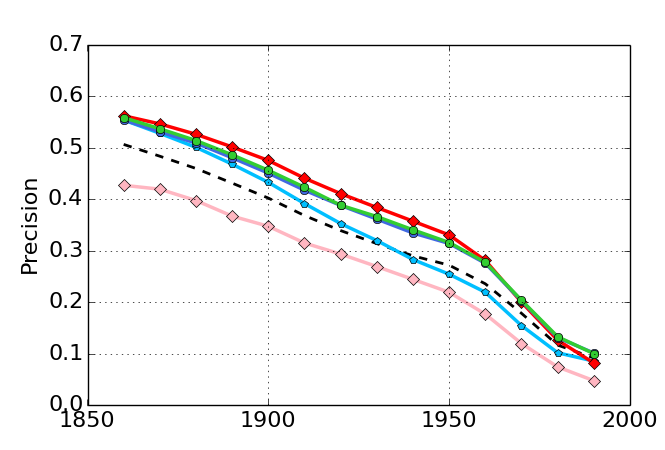
\includegraphics[width=.98\linewidth]{figures/GREWAL_precision_frq200_future.png}
  \caption{\sc Frq-200}
\end{subfigure}
\begin{subfigure}{.32\textwidth}
  \centering
  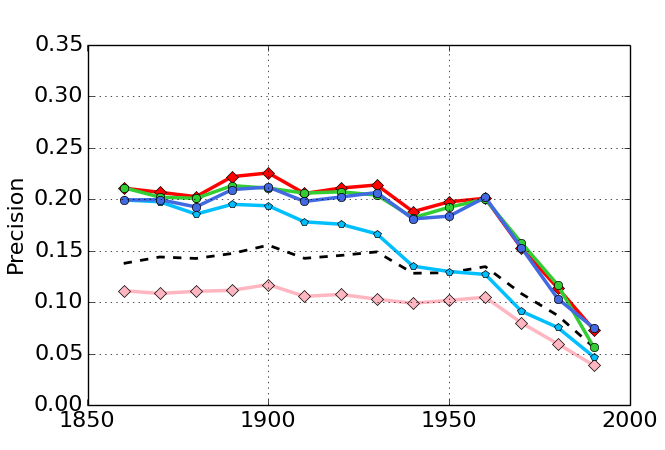
\includegraphics[width=.98\linewidth]{figures/GREWAL_precision_rand200.png}\\
  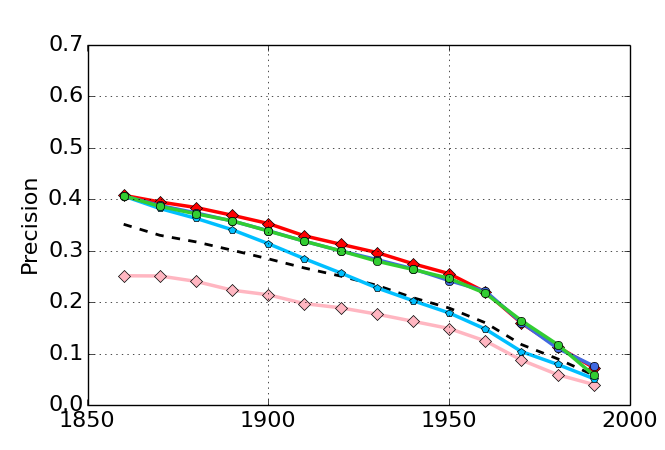
\includegraphics[width=.98\linewidth]{figures/GREWAL_precision_rand200_future.png}
  \caption{\sc Rand-200}
\end{subfigure}
\begin{subfigure}{.32\textwidth}
  \centering
  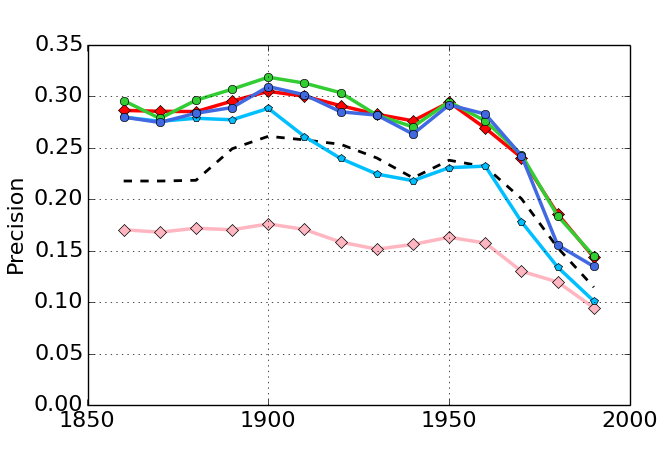
\includegraphics[width=.98\linewidth]{figures/GREWAL_precision_syn65.png}\\
  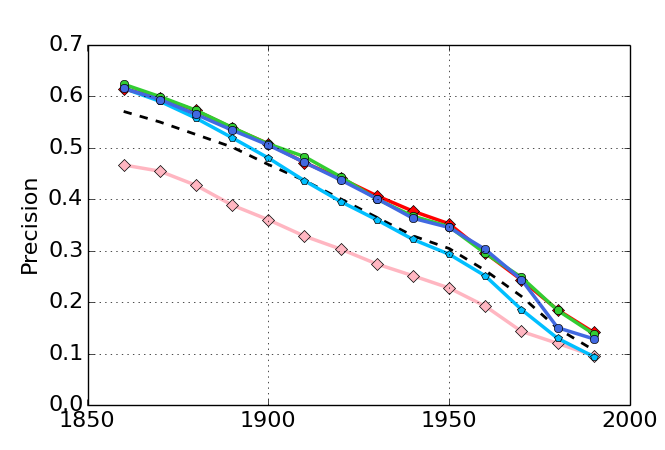
\includegraphics[width=.98\linewidth]{figures/GREWAL_precision_syn65_future.png}
  \caption{\sc Syn-65}
\end{subfigure}
\caption{Model predictive accuracy on the {\sc Frq-200}, {\sc Rand-200}, and {\sc Syn-65} adjective sets.
{\it Top row}: Predictive accuracy when only novel adjective-noun pairs in the following decade are considered.
{\it Bottom row}: Predictive accuracy when all future adjective extensions are considered.}
\label{fig:accuracy}
\end{figure}


Table \ref{table:modelpredexamples} provides some examples of model prediction and highlights the limitations of the approach. It is worth noting that while the exemplar model performed well in comparison to the other models, all models failed to predict parts of the empirical data. This issue might be partly due to the fact that our semantic representation of nouns is inadequate to capture the kinds of rich knowledge that determines adjective modification of nouns, and partly due to the historical events that add randomness to the process, e.g., how alcohol prohibition in the 1920s made {\it illegal} an appropriate adjective modifier for {\it alcohol}, and how {\it American} and {\it Vietnam} became associated in context presumably due to the Vietnam War around the 1960s.


\begin{table}
\small
\caption{Examples of model prediction on the {\sc Frq-200} adjective set.
Adjectives with an asterisk (*) indicate true positives retrieved by models.
We present predictions for nouns {\it cigarette}, {\it alcohol}, and {\it Vietnam} as the adjectives they first pair with in the 1880s, 1920s, and 1960s respectively reflect sentiment (e.g., {\it social cigarette}) or historic events (e.g., {\it illegal alcohol} due to prohibition, {\it American Vietnam} due to the Vietnam war).\label{table:modelpredexamples}}
\begin{tabularx}{\textwidth}{lQ}
\lsptoprule
noun \& decade & {\it cigarette}, 1880s \\
new adjectives & {\it better}, {\it modern}, {\it several}, {\it excessive}, {\it American}, {\it social} \\
baseline prediction & {\it original}, {\it particular}, {\it English}, {\it natural}, {\it perfect}, {\it modern}* (1/6) \\
exemplar prediction & {\it black}, {\it red}, {\it English}, {\it poor}, {\it original}, {\it particular} (0/6) \\
prototype prediction & {\it red}, {\it black}, {\it dry}, {\it warm}, {\it cold}, {\it English} (0/6) \\
10-NN prediction & {\it original}, {\it warm}, {\it particular}, {\it red}, {\it English}, {\it dry} (0/6) \\
\midrule
noun \& decade & {\it alcohol}, 1920s \\
new adjectives & {\it female}, {\it analogous}, {\it red}, {\it bitter}, {\it marked}, {\it illegal} \\
baseline prediction & {\it perfect}, {\it extraordinary}, {\it moral}, {\it physical}, {\it western}, {\it christian} (0/6) \\
exemplar prediction & {\it red}*, {\it moral}, {\it artificial}, {\it dense}, {\it perfect}, {\it marked}* (2/6) \\
prototype prediction & {\it artificial}, {\it perfect}, {\it marked}*, {\it red}*, {\it physical}, {\it moral} (2/6) \\
10-NN prediction & {\it red}*, {\it moral}, {\it dense}, {\it perfect}, {\it analogous}*, {\it artificial} (2/6) \\
\midrule
noun \& decade & {\it Vietnam}, 1960s \\
new adjectives & {\it western}, {\it tropical}, {\it eastern}, {\it colonial}, {\it particular}, {\it more}, {\it top}, {\it poor}, {\it American} \\
baseline prediction & {\it same}, {\it more}*, {\it great}, {\it particular}*, {\it American}*, {\it different}, {\it natural}, {\it human}, {\it English} (3/9) \\
exemplar prediction & {\it western}*, {\it eastern}*, {\it more}*, {\it particular}*, {\it great}, {\it colonial}*, {\it inner}, {\it same}, {\it poor}* (6/9) \\
prototype prediction & {\it great}, {\it same}, {\it western}*, {\it more}*, {\it American}*, {\it eastern}*, {\it particular}*, {\it European}, {\it French} (5/9) \\
10-NN prediction & {\it western}*, {\it eastern}*, {\it more}*, {\it tropical}*, {\it colonial}*, {\it great}, {\it better}, {\it inner}, {\it particular}* (6/9) \\
\lspbottomrule
\end{tabularx}
\end{table}

\subsection{Chaining in semantically changing and stable adjectives}\largerpage

We next examine the extent to which the chaining algorithms predict extensional patterns in both semantically changing and stable adjectives in history. Because the chaining view presumes meaning change to take incremental (as opposed to abrupt) steps, it is plausible that it is less effective in predicting adjective extension in those adjectives that show substantial change in meaning over time. However, if chaining reflects a generic mechanism of meaning change, we should expect the models described to predict both semantically changing and stable adjectives.

To investigate this issue, we performed a group comparison where we split each adjective set into two subsets: a semantically changing group that showed the highest degrees of semantic change, and a semantically stable group that showed the least degrees of semantic change. We defined the degree of semantic change of an adjective based on its semantic neighbourhood profiles during the flanking decades: 1850s and 1990s. We followed the same procedure as \citet{xu2015}, where we calculated the degree of overlap in 100 semantic neighbours in adjectives (using diachronic word embeddings from \citealp{hamilton-etal-2016-diachronic}) between the flanking decades and took the inverse of that quantity as degree of change: a fully stable adjective would have 100\% overlap in its neighbourhood, whereas a highly changing adjective would have low \% overlap in its neighbourhood. We then applied the same models of chaining to these two subgroups in each of the three adjective sets.\footnote{For the prototype model, we only present results based on the (moving) prototype model because it was shown to be a superior model than the progenitor model that assumes the prototype to be time-invariant, both in Section~\ref{sec:modeval} and \citet{habibi}.} 

We analyzed the 50 most and least changing adjectives from the {\sc Frq-200} and {\sc Rand-200} sets, and only 20 most and least changing adjectives from the {\sc Syn-65} set because it contained 61 adjectives in total. The results appear in Figure~\ref{fig:change-stable}. We observed that the proposed algorithms of chaining, particularly the exemplar, prototype, and 10-NN models, perform substantially better than the frequency baseline. This observation holds for both the semantically changing and stable adjective subgroups, suggesting that chaining mechanisms apply equally to these adjective sets. In both the {\sc Frq-200} and {\sc Rand-200} sets, the exemplar model consistently outperforms the alternative models in predictive accuracy over time, yet its performance is not the strongest in the {\sc Syn-65} (though this particular set has the smallest subset size of 20 adjectives). These results suggest that chaining is a generic mechanism in historical adjective extension.

\begin{figure}[p]
\begin{minipage}{\textwidth}
  \centering
  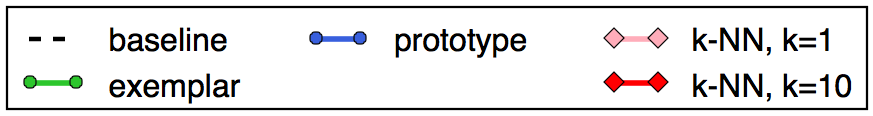
\includegraphics[width=.50\linewidth]{figures/GREWAL_legend_b.png}
\end{minipage}
\begin{center}
    \textsc{Frq-200}
\end{center}

\begin{minipage}{.5\textwidth}
  \centering
  50 least changed adjectives
  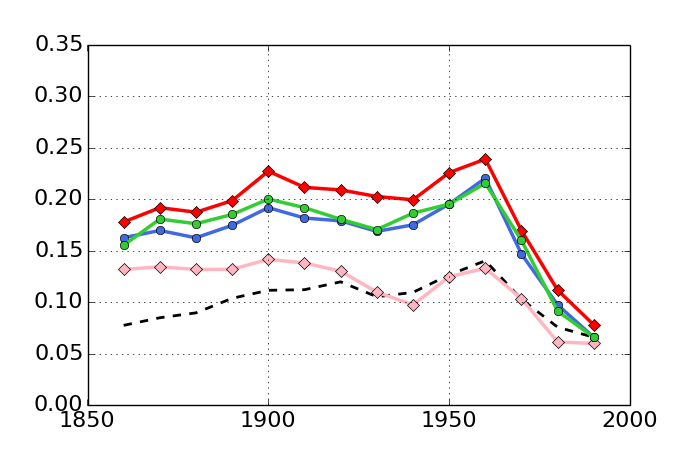
\includegraphics[width=.95\linewidth]{figures/GREWAL_frq200_least_changed.png}
\end{minipage}\begin{minipage}{.5\textwidth}
  \centering
  50 most changed adjectives
  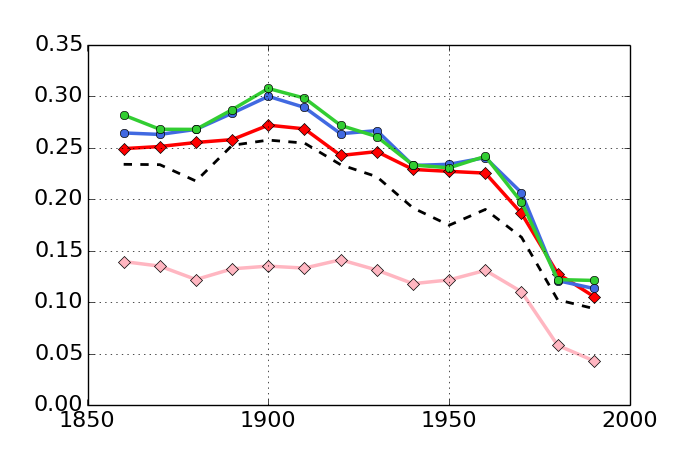
\includegraphics[width=.95\linewidth]{figures/GREWAL_frq200_most_changed.png}
\end{minipage}

\begin{center}
    \textsc{Rand-200}
\end{center}

\begin{minipage}{.5\textwidth}
  \centering
  50 least changed adjectives
  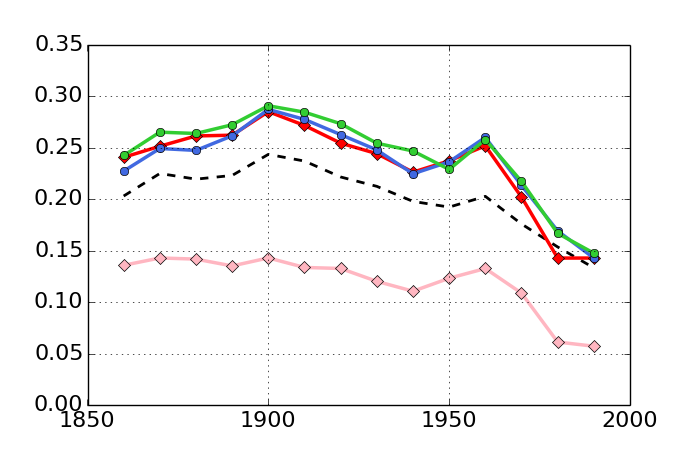
\includegraphics[width=.95\linewidth]{figures/GREWAL_rand200_least_changed.png}
\end{minipage}\begin{minipage}{.5\textwidth}
  \centering
  50 most changed adjectives
  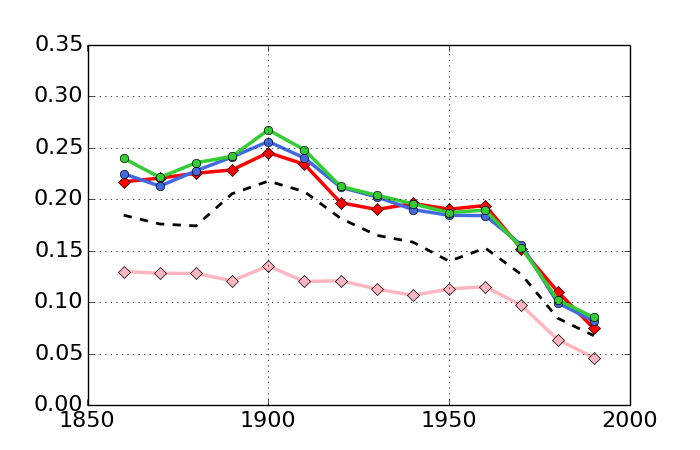
\includegraphics[width=.95\linewidth]{figures/GREWAL_rand200_most_changed.png}
\end{minipage}

\begin{center}
    \textsc{Syn-65}
\end{center}

\begin{minipage}{.5\textwidth}
  \centering
  20 least changed adjectives
  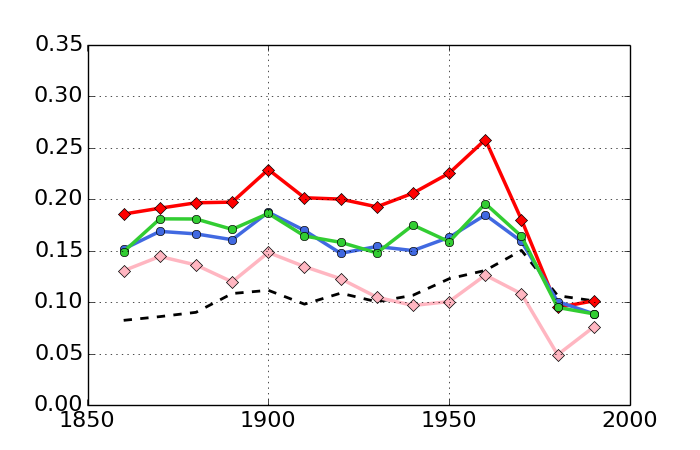
\includegraphics[width=.95\linewidth]{figures/GREWAL_syn65_least_changed.png}
\end{minipage}\begin{minipage}{.5\textwidth}
  \centering
  20 most changed adjectives
  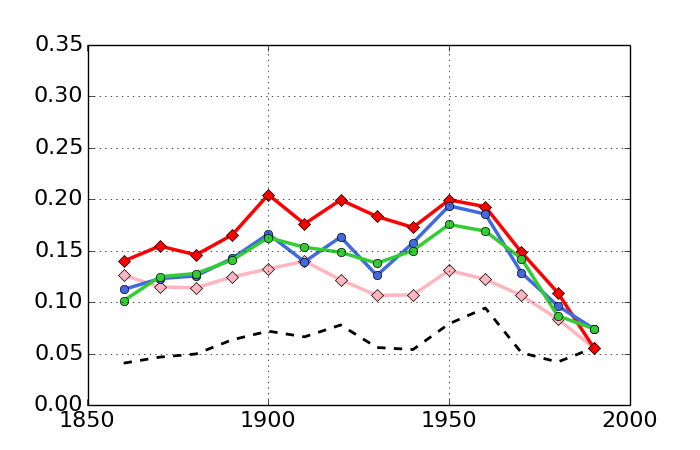
\includegraphics[width=.95\linewidth]{figures/GREWAL_syn65_most_changed.png}
\end{minipage}
\caption{Model predictive accuracy on the most semantically changing and stable adjectives from {\sc Frq-200}, {\sc Rand-200}, and {\sc Syn-65} adjective sets.}
\label{fig:change-stable}
\end{figure}



\section{Discussion}

Our findings support the overall hypothesis that semantic neighbourhood density influences how novel adjective-noun pairings emerge, although the distinction between the exemplar model and the alternative models is small for drawing strong conclusions from this initial investigation. Nevertheless, all the models we examined perform considerably better than the baseline model. Our work mirrors existing studies on chaining in the extension of grammatical categories~\citep{lakoff1987,bybee1994evolution,habibi}, and we discuss its limitations and implications toward a general theory of word meaning extension.

\subsection{Limitations}

Our formulation of chaining depends on semantic similarity. One drawback of this assumption is that although chaining mechanisms may retrieve nouns that are similar to a query noun, there is no independent mechanism of checking whether the adjective-noun pairing is plausible. That is, our implementation of chaining does not explicitly ``perform a check'' as to whether a predicted ad\-jec\-tive-noun pairing is sensible. As adjectives accumulate novel senses, the set of possible nouns they can pair with will also vary due to external factors orthogonal to the internal mechanism of chaining. Here we acknowledge this limitation and consider it an important future direction to explore the interaction of internal and external factors that co-shape word meaning extension and  semantic change.

Throughout our analyses we have assumed that distributed semantic representations, or word embeddings, are sufficient to capture the meaning of nouns. In particular, we used Word2Vec to capture distributional meaning of words from linguistic context, but other variants of semantic representation are available and should be considered in future explorations. Importantly, perceptual (e.g., visual) features might be especially relevant for constructing the meaning of concrete nouns, and our current construction of the semantic space might not capture these features.
There exists computational work that explores  adjective meaning using a combination of visual and linguistic information. For instance, \citet{lazaridou2015} applied cross-modal mappings between visual and linguistic representations to assign adjective labels to visual inputs, and \citet{nagarajan2018} followed up by learning a linear mapping that predicts adjective descriptors based on  visual input.
However, one limiting factor of these cross-modal approaches is that they may not be relevant to predicting adjective pairings with abstract nouns where perceptual grounding is more difficult to establish. In these cases, both socio-cultural factors and cognitive devices such as metaphor may be relevant in predicting adjective extension, above and beyond the semantic representation and the simple chaining mechanisms that we have considered. 

Our analyses have relied on written text (i.e., books) which might not be fully representative of natural language use that also involves colloquialism and conversations (represented more accurately in spoken text corpora). The interpretations we drew from our analyses are thus restricted to formal forms of language, although they are also useful reflections of conventional language use. Earlier work by \citet{williams1976} on synaesthetic adjectives has also used dictionaries as a source of investigation, and a potential research direction is to examine the properties of adjective meaning extension or change in both written and spoken text. Written language is likely to be a delayed reflection of spoken language, and as such we might expect changes in word meaning and usage in spoken language to precede those in written text. Colloquialism may also add nuances beyond this difference, whereby language use is notably more casual and flexible (partly due to the socio-cultural knowledge involved), e.g., emergent adjective usages in slang might be harder to predict in comparison to the case of formal written text.

\subsection{Relations of chaining and semantic change}

The proposal of semantic chaining as initially described by \citet{lakoff1987} has focused on the formation of complex linguistic categories, particularly grammatical classes such as classifiers and prepositions. Although Lakoff did not discuss extensively the relations of chaining and historical semantic change, the anecdotal cases that he described have assumed a connection between the chaining mechanism and the process of polysemy, or word sense extension. For instance, in both of his accounts on the extension of classifier systems and spatial prepositions, he described how polysemous extensions -- e.g., how Dyirbal classifiers group ideas related to women, fire, and dangerous things~\citep{lakoff1987}, and how English \textit{over} expresses a broad range of spatial configurations and metaphorical senses~\citep{lakoff1987,brugman88} -- might depend on image schematic transformations that are reflected through a process of chaining where one referent or sense links to another in complex chain-like structures. Recent computational work has extended these ideas in a formal setting and found that models of chaining -- similar to those described in this chapter -- can explain historical word sense extension in the English lexicon~\citep{ramiro2018}, although such models are far from perfect.

A caveat in both that study and \citegen{lakoff1987} work is the under-specification of the diverse knowledge involved in word meaning extension and semantic change, which is clearly beyond the embedding-based semantic representation presented here. In this respect, whether or how the theory of chaining can explain the diverse range of semantic change in adjectives and other word classes remains an important open question.


\subsection{Toward a general theory of word meaning extension}

The lexicon is an innovative product of the mind, and here we have focused on examining one critical form of lexical innovation that involves word meaning extension. A general account of word meaning extension in natural language ought to explain how it functions at different temporal scales not restricted to a historical setting.

There are at least three levels at which word meaning extension can occur, summarized in decreasing temporal scales: (1) across languages, the relics of word meaning extension are reflected in the colexification and polysemy structures that are likely a result of language evolution through tens of thousands of years~\citep{francois2008semantic,youn2016universal}, e.g., how a single word form like \textit{fire} can denote the senses of `physical fire', `flame', and `anger'; (2) within a language, word meaning extension can occur in language change during hundreds of years~\citep{sweetser91,traugott2001regularity}, e.g., how words like \textit{mouse} originally referred to `a type of rodent' later extended to express `a computer device'; (3) in child development typically within the first 2--3 years of life, children extend word meaning toward novel objects for which they lack the proper words in the form of overextension~\citep{vygotsky1962language,clark1978strategies,rescorla1980overextension}, e.g., how children use \textit{ball} to refer to `a balloon'. Characterizing the common mechanisms and knowledge underlying these phenomena will shed light on word meaning extension as a general strategy for making innovative use of a finite lexicon.

Recent studies have made initial progress toward this direction. For instance, \citet{ferreira} developed a multi-modal semantic framework based on the exemplar model of chaining and showed that it predicts children's overextension behavior in a variety of studies from the psychological and linguistic literature. \citet{xu2020conceptual} showed that the frequency variation in cross-linguistic colexification, i.e., why certain senses are more commonly grouped (e.g., `fire'--`flame') under a single word form than others (e.g., `fire'--`anger') can be explained by a principle of cognitive economy, whereby senses that are frequently colexified across languages tend to be easily associable -- an argument that is consistent with the chaining account presented here. However, there is a critical lack of demonstrating how the approaches and principles identified in language development and cross-linguistic settings can also explain historical semantic change attested in the world's languages.

We believe that a general formal account of word meaning extension will involve three key ingredients related to the chaining processes discussed in this chapter: (1) algorithmic formulations such as the exemplar model described that capture the  mechanisms of semantic chaining; (2) rich knowledge structures that support these mechanisms toward a diverse range of extensional strategies such as metonymy and metaphor; (3) external socio-cultural influences or events that provide the driving force for word meaning extension.

\section{Conclusion}

We have presented a computational approach to explore regularities in the historical composition of adjectives and nouns through probabilistic models of chaining. Our approach provides clues to the generative mechanisms that give rise to novel adjective usages over time, and we hope it will stimulate future work on the semantic representation and the interaction of cognitive and socio-cultural underpinnings of word meaning extension and semantic change.




\section*{Acknowledgements}
We thank Barend Beekhuizen, Lars Borin, Sammy
Floyd, Adam Jatowt, Charles Kemp, and Nina Tahmasebi for helpful discussion and constructive comments. We also thank Amir Ahmad Habibi for sharing data and code. KG is supported by a Bell Graduate Scholarship and a Vector Scholarship in Artificial Intelligence. YX is funded through an NSERC Discovery Grant RGPIN-2018-05872 and a SSHRC Insight Grant \#435190272.

\section*{Abbreviations}
\begin{tabularx}{\textwidth}{@{}lQ@{}}
NN & nearest-neighbour
\end{tabularx}


\appendixsection{Adjective sets}

Here we present all adjectives used in our analysis, namely from the {\sc Frq-200}, {\sc Rand-200}, and {\sc Syn-65} adjective sets.
Adjectives with an asterisk (*) are included in at least two of the three adjective sets.
The first table gives the adjectives that constitute {\sc Syn-65}, and we note two important details about this set.
First, the set of synaesthetic adjectives proposed by \citet{williams1976} actually contains 64 unique adjectives as {\it light} is repeated.
Second, the Google Books corpus ties all tokens to words in WordNet, and since {\it acrid}, {\it aspre}, and {\it tart} (all synaesthetic adjectives) are not WordNet adjectives, we could not reliably measure their uses through time.
For this reason, we excluded these from {\sc Syn-65} and have 61 adjectives in total, listed in Table~\ref{tab:synadjs}.

\begin{table}\footnotesize
\caption{List of 61 adjectives in {\sc Syn-65}.\label{tab:synadjs}
Adjectives with an asterisk (*) appear in at least one of {\sc Frq-200} and {\sc Rand-200} as well.}
\begin{tabular}{ *{7}{>{\itshape}l} }
\lsptoprule
\multicolumn{7}{c}{\normalfont\scshape Syn-65}\\
\midrule
acute & cloying & dulcet* & grave & light & quiet & sour \\
austere & coarse & dull & hard & little & rough & strident \\
big & cold* & eager & harsh & loud & shallow & sweet \\
bitter* & cool & empty & heavy & low & sharp & thick \\
bland & crisp & even & high & mellow & shrill & thin \\
bright & dark & faint & hollow & mild & small & vivid \\
brilliant* & deep & fat & hot & piquant & smart & warm* \\
brisk & dim & flat & keen & poignant & smooth & \\
clear & dry* & full & level & pungent & soft & \\
\lspbottomrule
\end{tabular}
\end{table}

Next, we present the {\sc Frq-200} and {\sc Rand-200} adjective sets and the clusters we used for the analysis, listed in Table~\ref{adjclusters}.
Since these two sets draw adjectives from identical clusters, we present the two adjective sets so we can easily compare adjectives drawn from same cluster between the two sets.

{\scriptsize\begin{longtable}{ *{6}{>{\itshape}l}}
\caption{Lists of adjectives and clusters in {\sc Frq-200} and {\sc Rand-200}.\label{adjclusters}}\\
\lsptoprule\endfirsthead\midrule\endhead\endfoot\lspbottomrule\endlastfoot
\multicolumn{2}{c}{cluster 1 of 20} & \multicolumn{2}{c}{cluster 2 of 20} & \multicolumn{2}{c}{cluster 3 of 20} \\
{\normalfont\scshape Frq-200} & {\normalfont\scshape Rand-200} & {\normalfont\scshape Frq-200} & {\normalfont\scshape Rand-200} & {\normalfont\scshape Frq-200} & {\normalfont\scshape Rand-200} \\
\midrule
casual &  amiable &  bare &  contorted &  sufficient &  alterable\\
eccentric &  chatty &  curly &  dainty &  analogous &  contemporaneous\\
energetic &  communicative &  eyed &  furrowed &  equal &  reconcilable\\
entertaining &  fiery &  female &  hale &  calculable &  chargeable\\
enthusiastic &  fluent &  feminine &  horny* &  receivable &  distributive\\
forgiving &  guileless &  horny* & limber &  derived &  accessary\\
glib &  lovable &  male &  sage &  binding &  lineal\\
intelligent &  loyal &  naked &  skeletal* &  indirect &  allotted\\
passionate &  patriotic &  pale &  smoky &  undivided &  noncommercial\\
polite &  unorthodox &  skeletal* &  swaggering &  eligible &  classifiable\\
\midrule
\multicolumn{2}{c}{cluster 4 of 20} & \multicolumn{2}{c}{cluster 5 of 20} & \multicolumn{2}{c}{cluster 6 of 20} \\
{\normalfont\scshape Frq-200} & {\normalfont\scshape Rand-200} & {\normalfont\scshape Frq-200} & {\normalfont\scshape Rand-200} & {\normalfont\scshape Frq-200} & {\normalfont\scshape Rand-200} \\
\midrule
cold* &  chilly &  algebraic &  binary &  blind &  intact\\
dense &  cold* &  conventional &  biotic &  impossible &  irretrievable\\
dry* &  drizzling &  discrete &  crystalline &  incomplete &  malfunctioning\\
eastern &  encroaching &  electrical &  fusible &  isolated &  obscure\\
hardy &  fertile &  microscopic &  geometric &  pregnant &  overlooked\\
northern &  funicular &  multicellular &  interfacial &  scarce &  powerless\\
south &  homeward &  predictive &  modular &  silent &  unmarked\\
tropical &  littoral &  rotational &  perceptual &  submerged &  unstable\\
warm* &  unincorporated &  thermal &  refrigerant &  unknown &  unstudied\\
western &  watery &  volcanic &  stratified &  unrelated &  valueless\\
\midrule
\multicolumn{2}{c}{cluster 7 of 20} & \multicolumn{2}{c}{cluster 8 of 20} & \multicolumn{2}{c}{cluster 9 of 20} \\
{\normalfont\scshape Frq-200} & {\normalfont\scshape Rand-200} & {\normalfont\scshape Frq-200} & {\normalfont\scshape Rand-200} & {\normalfont\scshape Frq-200} & {\normalfont\scshape Rand-200} \\
\midrule
appropriate &  complex &  alien &  antipodal &  everyday &  approaching\\
balanced &  delighted &  colonial &  congruous &  firm &  descending\\
basic &  foolproof &  divine &  dynastic &  more &  fiddling\\
better &  grateful &  heavenly &  hierarchical &  original &  former\\
different &  intensive &  human &  invariable &  particular &  intensifying\\
natural &  knowledgeable &  inner &  overt &  physical &  probable\\
positive &  livable &  medieval &  paschal &  preliminary &  rental\\
solid &  realistic &  modern &  protestant &  same &  reverse\\
superior &  structured &  moral &  recessive &  several &  sliding\\
sure &  varied &  philosophical &  sacred &  top &  thirteenth\\
\midrule
\multicolumn{2}{c}{cluster 10 of 20} & \multicolumn{2}{c}{cluster 11 of 20} & \multicolumn{2}{c}{cluster 12 of 20} \\
{\normalfont\scshape Frq-200} & {\normalfont\scshape Rand-200} & {\normalfont\scshape Frq-200} & {\normalfont\scshape Rand-200} & {\normalfont\scshape Frq-200} & {\normalfont\scshape Rand-200}\\
\midrule
allergic &  carcinogenic &  black &  ceramic &  bent &  hysterical\\
antibiotic &  coagulate &  circular &  cyclopean &  bourgeois &  inattentive\\
artificial &  colorless &  concave &  fireproof &  corrupt &  irreligious\\
dietary &  milky &  crimson &  legible &  disreputable &  lunatic\\
fibrous &  nonfat &  distinctive &  rectilinear &  domineering &  opportunist\\
liquid &  pulpy &  fluorescent &  sleek &  evil &  parochial\\
mucous &  scented &  incised &  tucked &  fascist &  possessive\\
powdery &  spongy &  red &  umber &  jugular &  resentful\\
raw &  steamed &  tubular &  unglazed &  pious &  uncongenial\\
synthetic &  vanilla &  white &  Venetian &  warlike &  unengaged\\
\midrule
\multicolumn{2}{c}{cluster 13 of 20} & \multicolumn{2}{c}{cluster 14 of 20} & \multicolumn{2}{c}{cluster 15 of 20} \\
{\normalfont\scshape Frq-200} & {\normalfont\scshape Rand-200} & {\normalfont\scshape Frq-200} & {\normalfont\scshape Rand-200} & {\normalfont\scshape Frq-200} & {\normalfont\scshape Rand-200} \\
\midrule
bitter* &  brokenhearted & affected & bottomed & abusive & appalling\\
debilitating & confused & buried & credited & deplorable & bias\\
emotional & delirious & distributed & jammed & exaggerated & capricious\\
hopeless & disturbed & given & owned & excessive & exorbitant\\
odd* &  odd* &  left & rose & illegal & hostile\\
poor & patchy & marked & scattered* &  simplistic & imprecise\\
troubled & regretful & modified & settled & undue & inelegant\\
unhappy* &  thirsty & scattered* &  shattered & unintentional & innocuous\\
weird & unhappy* &  used & surrounded & unproductive & unbalanced\\
worst & untidy & worn & sworn & wrong & unsound\\
\midrule
\multicolumn{2}{c}{cluster 16 of 20} & \multicolumn{2}{c}{cluster 17 of 20} & \multicolumn{2}{c}{cluster 18 of 20}\\
{\normalfont\scshape Frq-200} & {\normalfont\scshape Rand-200} & {\normalfont\scshape Frq-200} & {\normalfont\scshape Rand-200} & {\normalfont\scshape Frq-200} & {\normalfont\scshape Rand-200}\\
\midrule
adrenal & cesarean & American & Arabian & brilliant* &  adored\\
alveolar & endoscopic & Asian & Catalan & conspicuous & commanding\\
bivariate & hemorrhagic & Christian & Chinese & ecstatic & fantastic\\
cardiovascular & hyoid & Dutch* &  Cornish & extraordinary & favorite\\
clinical & intervertebral & English & Dutch* &  fitting & gallant\\
diagnostic & lobular & European & Haitian & great & halcyon\\
neural & monovalent & French & Hungarian & incomparable & loved\\
peritoneal & normotensive & Roman & Kurdish & perfect & superb\\
spinal & valved & Serbian & Taiwanese & singular & tragic\\
ulcerative & vesicular & Spanish & Thai & startling & undefeated\\
\midrule
\multicolumn{2}{c}{cluster 19 of 20} & \multicolumn{2}{c}{cluster 20 of 20}\\
{\normalfont\scshape Frq-200} & {\normalfont\scshape Rand-200} & {\normalfont\scshape Frq-200} & {\normalfont\scshape Rand-200}\\
\cmidrule[0.5pt]{1-4}
budgetary & agrarian & aesthetic & clarion\\
civil & catechetical & artistic & contemporary\\
criminal & clandestine & classical & darkling\\
marital & constitutional & clever & dulcet* \\
mental & curricular & colloquial & earthy\\
national & hourly & dreamy & falsetto\\
nuclear & intramural & hilarious & longhand\\
parental & qualitative & intimate & ponderous\\
regional & recreational & narrative & soothing\\
social & sectional & rhetorical & wry\\
\end{longtable}}

\appendixsection{Temporal trends in model precision}

As discussed in the main text, the model precision generally decreases across all models with time. As Figure \ref{fig:number_of_new_pairs} shows, the average number of nouns to predict in each decade decreases with time.
This trend applies to both sets of true positives: only adjectives that first co-occur with a given noun $n^*$ in decade $t + \Delta$, and also in any future decade.
Consequently, the precision falls systematically in later decades because there are fewer novel pairings to predict in the data. 


\begin{figure}
\begin{minipage}{\textwidth}
  \centering
  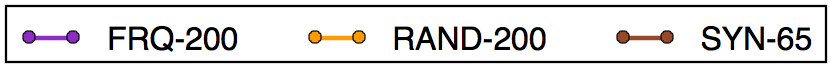
\includegraphics[width=.50\linewidth]{figures/GREWAL_legend_dataset.png}
\end{minipage}

\begin{subfigure}[b]{.48\textwidth}
  \centering
  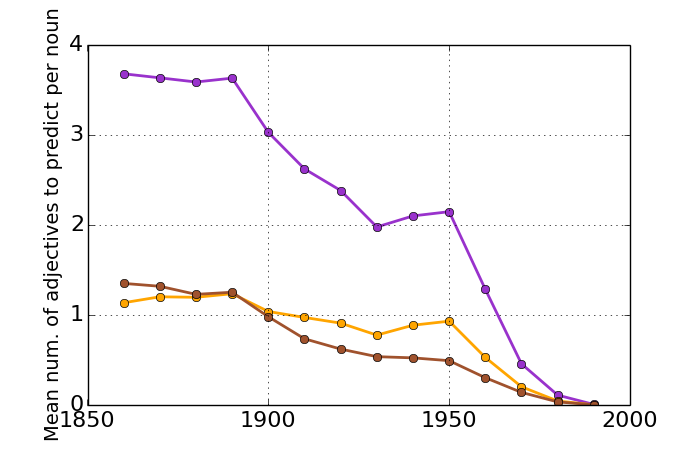
\includegraphics[width=.96\linewidth]{figures/GREWAL_number_of_pairs_to_predict.png}
  \caption{In decade $t + \Delta$}
\end{subfigure}\begin{subfigure}[b]{.48\textwidth}
  \centering
  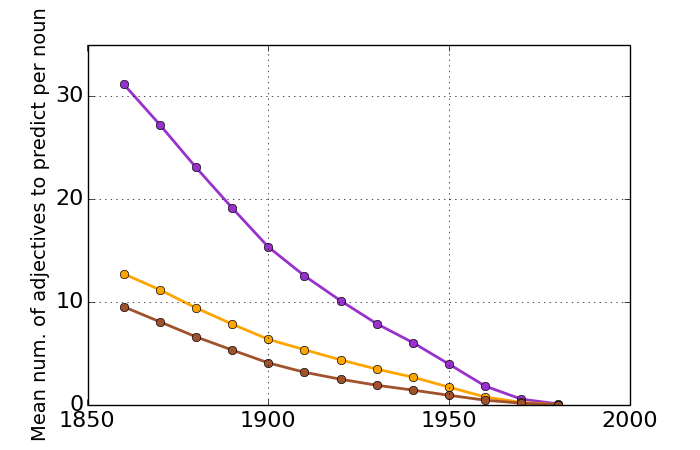
\includegraphics[width=.96\linewidth]{figures/GREWAL_number_of_pairs_to_predict_future.png}
  \caption{In any future decade $t' > t$}
\end{subfigure}
\caption{The average number of novel adjective-noun pairs remaining for each model to predict across all times and adjective sets.
This value is computed across all nouns for which a predictive model makes adjective prediction.
\label{fig:number_of_new_pairs}}
\end{figure}
\clearpage

\appendixsection{Semantically changing and stable adjectives}

\begin{footnotesize}
\begin{longtable}{ll}
\caption{Lists of most and least changed adjectives from the {\sc Frq-200}, {\sc Rand-200}, and {\sc Syn-65} sets, along with their top semantic neighbours during initial (1850s) and terminal (1990s) periods of investigation.} \label{table:examples} \\\lsptoprule\endfirsthead\endhead\endfoot\lspbottomrule\endlastfoot
\multicolumn{2}{c}{{{\sc Frq-200}}} \\
\multicolumn{1}{c}{{Least Changed}} & \multicolumn{1}{c}{{Most Changed}} \\\midrule
1. {\it eccentric} & 1. {\it classical} \\
\qquad 1850s: {\it versatile}, {\it droll}, {\it impulsive} & \qquad 1850s: {\it theological}, {\it modern}, {\it greek} \\
\qquad 1990s: {\it incoherent}, {\it perverse}, {\it exquisite} & \qquad 1990s: {\it greek}, {\it traditional}, {\it contemporary} \\
& \\
2. {\it casual} & 2. {\it rhetorical} \\
\qquad 1850s: {\it occasional}, {\it trivial}, {\it careless} & \qquad 1850s: {\it idiomatic}, {\it didactic}, {\it fanciful} \\
\qquad 1990s: {\it careless}, {\it informal}, {\it friendly} & \qquad 1990s: {\it poetic}, {\it epistolary}, {\it grammatical} \\
& \\
3. {\it polite} & 3. {\it colloquial} \\
\qquad 1850s: {\it affable}, {\it hospitable}, {\it elegant} & \qquad 1850s: {\it imaginative}, {\it analytic}, {\it bewitching} \\
\qquad 1990s: {\it respectful}, {\it friendly}, {\it agreeable} & \qquad 1990s: {\it epistolary}, {\it poetic}, {\it idiomatic} \\
& \\
4. {\it intelligent} & 4. {\it narrative} \\
\qquad 1850s: {\it honest}, {\it rational}, {\it inquisitive} & \qquad 1850s: {\it detailed}, {\it circumstantial}, {\it brief} \\
\qquad 1990s: {\it clever}, {\it energetic}, {\it minded} & \qquad 1990s: {\it autobiographical}, {\it biblical}, {\it historical} \\
& \\
5. {\it enthusiastic} & 5. {\it artistic} \\
\qquad 1850s: {\it irrepressible}, {\it impulsive}, & \qquad 1850s: {\it scientific}, {\it architectural}, {\it literary} \\
\qquad {\it passionate} & \\
\qquad 1990s: {\it ardent}, {\it sincere}, {\it generous} & \qquad 1990s: {\it intellectual}, {\it musical}, {\it poetic} \\ \midrule
\multicolumn{2}{c}{{{\sc Rand-200}}} \\
\multicolumn{1}{c}{{Least Changed}} & \multicolumn{1}{c}{{Most Changed}} \\\midrule
1. {\it fluent} & 1. {\it contemporary} \\
\qquad 1850s: {\it versatile}, {\it idiomatic}, {\it sprightly} & \qquad 1850s: {\it recorded}, {\it voluminous}, {\it anonymous} \\
\qquad 1990s: {\it spoken}, {\it speaking}, {\it Arabic} & \qquad 1990s: {\it literary}, {\it historical}, {\it classical} \\
& \\
2. {\it amiable} & 2. {\it earthy} \\
\qquad 1850s: {\it humane}, {\it affable}, {\it estimable} & \qquad 1850s: {\it alkaline}, {\it gelatinous}, {\it nitrogenous} \\
\qquad 1990s: {\it dignified}, {\it virtuous}, {\it pleasing} & \qquad 1990s: {\it ceremonious}, {\it ravaging}, {\it disused} \\
& \\
3. {\it patriotic} & 3. {\it soothing} \\
\qquad 1850s: {\it loyal}, {\it disinterested}, {\it enlightened} & \qquad 1850s: {\it melancholy}, {\it sweet}, {\it sympathetic} \\
\qquad 1990s: {\it democratic}, {\it civic}, {\it loyal} & \qquad 1990s: {\it calm}, {\it sweet}, {\it shrill} \\
& \\
4. {\it fiery} & 4. {\it ponderous} \\
\qquad 1850s: {\it fierce}, {\it resistless}, {\it malign} & \qquad 1850s: {\it huge}, {\it cased}, {\it jingling} \\
\qquad 1990s: {\it mutinous}, {\it treacherous}, {\it fierce} & \qquad 1990s: {\it glistening}, {\it ethereal}, {\it noiseless} \\
& \\
5. {\it communicative} & 5. {\it clandestine} \\
\qquad 1850s: {\it sociable}, {\it choleric}, {\it affable} & \qquad 1850s: {\it nefarious}, {\it illicit}, {\it adulterous} \\
\qquad 1990s: {\it symbolic}, {\it verbal}, {\it functional} & \qquad 1990s: {\it disfigured}, {\it patrician}, {\it sedate} \\\midrule
\multicolumn{2}{c}{{{\sc Syn-65}}} \\
\multicolumn{1}{c}{{Least Changed}} & \multicolumn{1}{c}{{Most Changed}} \\\midrule
1. {\it bitter} & 1. {\it shrill} \\
\qquad 1850s: {\it astringent}, {\it sweet}, {\it poignant} & \qquad 1850s: {\it blithe}, {\it deafening}, {\it inaudible} \\
\qquad 1990s: {\it sour}, {\it harsh}, {\it intense} & \qquad 1990s: {\it pitched}, {\it startled}, {\it muffled} \\
2. {\it bland} & 2. {\it small} \\
\qquad 1850s: {\it mild}, {\it unobtrusive}, {\it affable} & \qquad 1850s: {\it smaller}, {\it size}, {\it sized} \\
\qquad 1990s: {\it unconverted}, {\it unadorned}, {\it affable} & \qquad 1990s: {\it sized}, {\it smaller}, {\it insignificant} \\
3. {\it coarse} & 3. {\it mellow} \\
\qquad 1850s: {\it dirty}, {\it threadbare}, {\it boned} & \qquad 1850s: {\it lustrous}, {\it chilly}, {\it balmy} \\
\qquad 1990s: {\it thin}, {\it fine}, {\it stiff} & \qquad 1990s: {\it perfumed}, {\it fragrant}, {\it sportive} \\
4. {\it cold} & 4. {\it austere} \\
\qquad 1850s: {\it clammy}, {\it wet}, {\it hot} & \qquad 1850s: {\it unsocial}, {\it disdainful}, {\it rigid} \\
\qquad 1990s: {\it warm}, {\it damp}, {\it windy} & \qquad 1990s: {\it matchless}, {\it apposite}, {\it erudite} \\
5. {\it cool} & 5. {\it pungent} \\
\qquad 1850s: {\it calm}, {\it chilly}, {\it warm} & \qquad 1850s: {\it juicy}, {\it ductile}, {\it astringent} \\
\qquad 1990s: {\it damp}, {\it hot}, {\it dry} & \qquad 1990s: {\it mown}, {\it fresh}, {\it colorless} \\
\end{longtable}
\end{footnotesize}

{\sloppy\printbibliography[heading=subbibliography,notkeyword=this]}
\end{document}
